\begin{figure}[t]
	\begin{minipage}[b]{0.49\linewidth}
		\centering
		\centerline{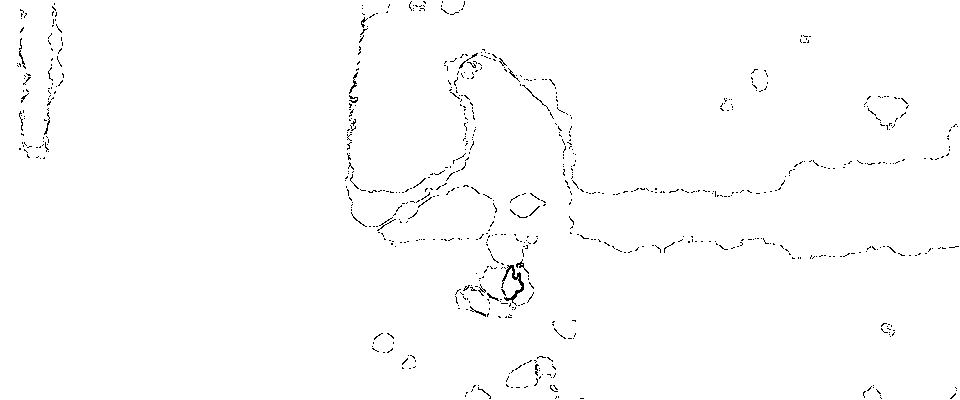
\includegraphics[width=\textwidth]{disparity_contours} }
		\centerline{\scriptsize{(a) Edges extracted from disparity map}}\medskip
	\end{minipage}
	\begin{minipage}[b]{0.49\linewidth}
		\centering
		\centerline{ 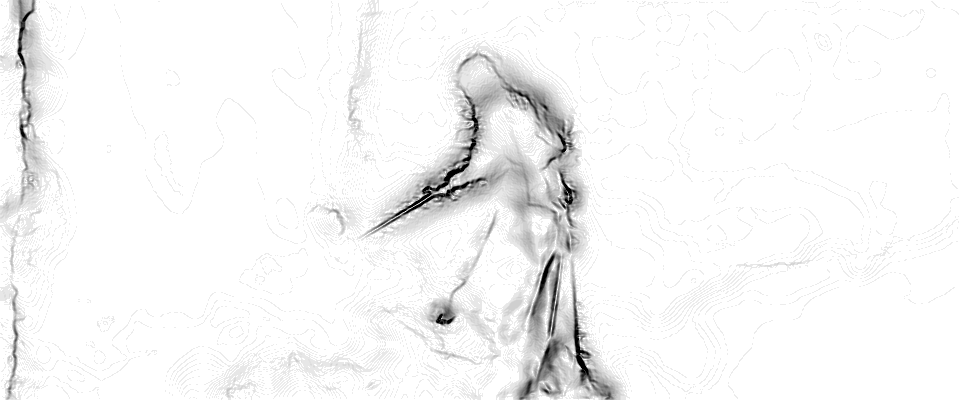
\includegraphics[width=\textwidth]{drop_contours} }
		\centerline{\scriptsize{(b) Edges extracted from motion-strength map }}\medskip
	\end{minipage}
	\hfill
	\begin{minipage}[b]{0.49\linewidth}
		\centering
		\centerline{ 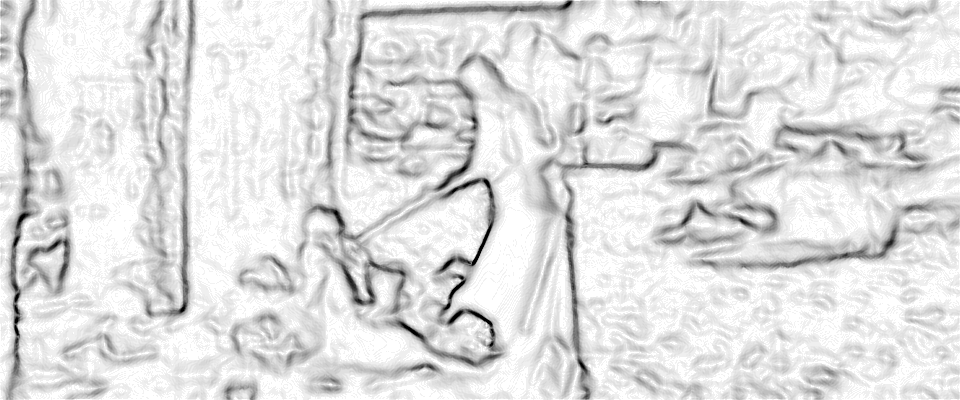
\includegraphics[width=\textwidth]{src_contours} }
		\centerline{\scriptsize{(c) Edges extracted from source frame}}\medskip
	\end{minipage}
	\hfill
	\begin{minipage}[b]{0.49\linewidth}
		\centering
		\centerline{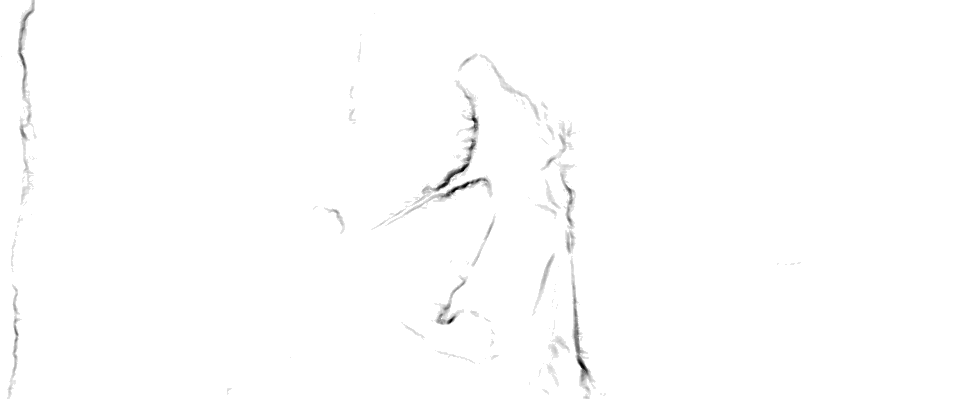
\includegraphics[width=\textwidth]{dfm_contours} }
		\centerline{\scriptsize{(d) Intersection of source and motion edges}}\medskip
	\end{minipage}
	\begin{minipage}[b]{\linewidth}
    \caption{Edges extracted from the disparity map~(a), filtered motion-strength
        map~(b), and source frame filtered using a scale-aware method~(c). The
        intersection of the motion and source-frame edge maps appears in~(d).}
    \label{fig:edges}
    \end{minipage}
\end{figure}
